\chapter{Grundlagen}%
\label{cha:essentials}

\section{Binarisierung}%
\label{sec:essentials_binarization}

Die Binarisierung ist eine Spezialform der sogenannten Segmentierung eines Bildes.
Während bei der allgemeinen Segmentierung das Bild generell in eine beliebige, aber finite, Anzahl von Regionen aufgeteilt wird, bezieht sich die Binarisierung konkret auf die Partitionierung in exakt zwei Teile.
Üblicherweise wird hierbei ein Graustufen- beziehungsweise Schwarzweißbild in ein Binärbild umgewandelt, mit dem Ziel das Bild in Hinter- und Vordergrund beziehungsweise Schwarz und Weiß aufzuteilen.

Die einfachste und am häufigsten verwendete Variante ist das sogenannte \enquote{Schwellenwertverfahren}.
Angenommen folgende Definitionen gelten:

\begin{tabu}{lX}
    \(P(x,y)\) & Graustufenwert an der Stelle \((x,y)\) \\
    \(P'(x,y)\) & Resultierender Binärwert an der Stelle \((x,y)\) \\
    \(T(x,y)\) & Schwellenwert an der Stelle \((x,y)\)
\end{tabu}

Dann ist das \enquote{Schwellenwertverfahren} definiert als:
\begin{gather}
    P'(x,y) = \begin{cases}
        \text{schwarz} & \text{wenn } P(x,y) < T(x,y) \\
        \text{weiß} & \text{ansonsten}
    \end{cases}
\end{gather}

Für die konkrete Schwellenwertfunktion steht eine große Auswahl an Definitionen zur Verfügung~\cite{DBLP:journals/jei/SezginS04}.
Generell lassen sich jedoch die Algorithmen in zwei Arten aufteilen: Globale und Lokale.
Erstere berechnen einen konstanten Schwellenwert \(T(x,y) = k\), welcher \enquote{global} auf die gesamte Grafik angewendet wird.
Letztere hingegen berechnen den Schwellenwert separat für jede Stelle \((x,y)\) anhand von in der \enquote{lokalen} Umgebung vorkommenden Statistiken.

Aufgrund dieser Eigenschaft sind lokale Schwellenwertfunktionen in der Lage, auch bei ungleichmäßiger Ausleuchtung des Bilds zufriedenstellende Ergebnisse zu liefern, da es der Funktion erlaubt wird, sich den lokal ändernden Gegebenheiten des Bilds anzupassen.
Dies erhöht jedoch signifikant den Rechenaufwand, da die Schwelle nicht nur ein einzelnes Mal, sondern für jedes Pixel neu berechnet werden muss.
Ein weiteres Problem ist der Umstand, dass eine passende Größe der \enquote{lokalen Umgebung}, beziehungsweise der Fenstergröße, gewählt werden muss.
Ist die Fenstergröße zu klein, so kann dies die Statistik verfälschen und zu optisch stark inkorrekten Ergebnissen führen.
Ist sie hingegen zu groß so steigt der Rechenaufwand entsprechend signifikant.
Auch die Fähigkeit zur Anpassung an neue Gegebenheiten des Bilds wird hierdurch abgeschwächt.

Globale Schwellenwertfunktionen unterliegen keinen solchen Einschränkungen, weshalb sie in der Regel bei einem geringeren Rechenaufwand bessere Ergebnisse erzielen, sofern die entsprechenden Grafiken keine Binarisierung benötigen, die sich lokalen Gegebenheiten anpassen muss.
Dies ist zum Beispiel in der Regel der Fall für annähernd saubere Aufnahmen von Textdokumenten, welche sich bereits optisch klar in Schwarz und Weiß aufteilen lassen.

\autoref{fig:essentials_binarization_uneven_illumination} zeigt die Vorteile lokaler Schwellenwertfunktionen exemplarisch an ihrer Anpassungsfähigkeit bei ungleichmäßiger Ausleuchtung.
Dem gegenüber steht unter anderem der Nachteil der finiten Fenstergröße in \autoref{fig:essentials_binarization_window_size}.
Da diese in der Abbildung zu Demonstrationszwecken bewusst kleiner als die Breite des Person gewählt wurde, passt sich die Schwellenwertfunktion der dunklen Farbe der Jacke an und senkt die lokal zu erreichende Schwelle.
Hierdurch erscheint der Großteil des Person fälschlicherweise Weiß und nur noch die lokalen, tiefschwarzen Extrema erscheinen dann Schwarz.

Im Entwurf (siehe \autoref{cha:theory}) wird die letztendliche Wahl auf Sauvola's Methode~\cite{DBLP:journals/pr/SauvolaP00} fallen.
Diese erzielt gute Ergebnisse in der Binarisierung von Textdokumenten~\cite{DBLP:journals/jei/SezginS04} und ist als lokale Schwellenwertfunktion ein passender Algorithmus für Fotografien bei natürlichem Licht mit ungleichmäßiger Ausleuchtung, so wie es im späteren Einsatz in einer Anwendung für Mobilgeräte der Fall sein wird.
Im nachfolgenden Abschnitt wird Sauvola's Methode näher erläutert.

\begin{figure}
    \begin{subfigure}[t]{0.3\textwidth}
        \centering
        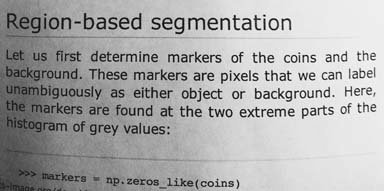
\includegraphics[interpolate=true,width=\textwidth]{images/essentials_binarization_uneven_illumination}
        \caption{Ursprüngliche Grafik~\cite{scikit-image}}%
    \end{subfigure}
    \hfill
    \begin{subfigure}[t]{0.3\textwidth}
        \centering
        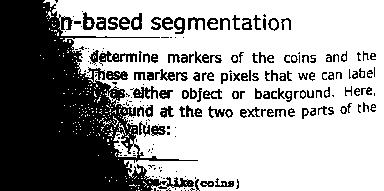
\includegraphics[interpolate=true,width=\textwidth]{images/essentials_binarization_uneven_illumination_otsu}
        \caption{Otsu's Methode\\(Global)}%
    \end{subfigure}
    \hfill
    \begin{subfigure}[t]{0.3\textwidth}
        \centering
        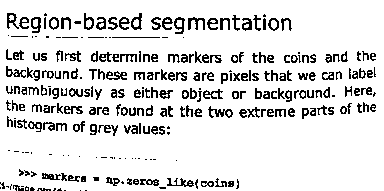
\includegraphics[interpolate=true,width=\textwidth]{images/essentials_binarization_uneven_illumination_sauvola}
        \caption{Sauvola's Methode\\(Lokal)}%
    \end{subfigure}
    \caption{Anpassungsfähigkeit lokaler Schwellenwertfunktionen bei ungleichmäßiger Ausleuchtung}%
    \label{fig:essentials_binarization_uneven_illumination}
\end{figure}

\begin{figure}
    \begin{subfigure}[t]{0.3\textwidth}
        \centering
        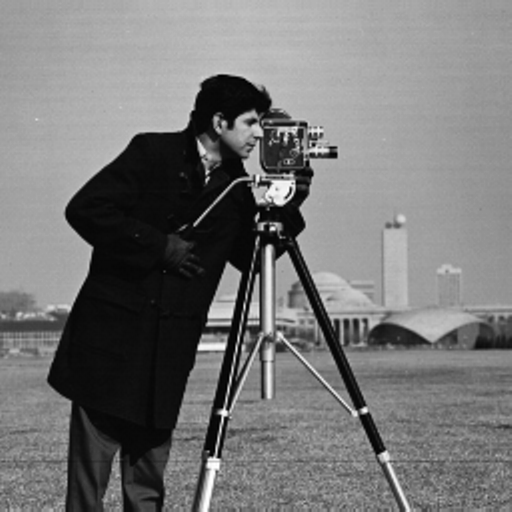
\includegraphics[interpolate=true,width=\textwidth]{images/essentials_binarization_window_size}
        \caption{Ursprüngliche Grafik~\cite{scikit-image}}%
    \end{subfigure}
    \hfill
    \begin{subfigure}[t]{0.3\textwidth}
        \centering
        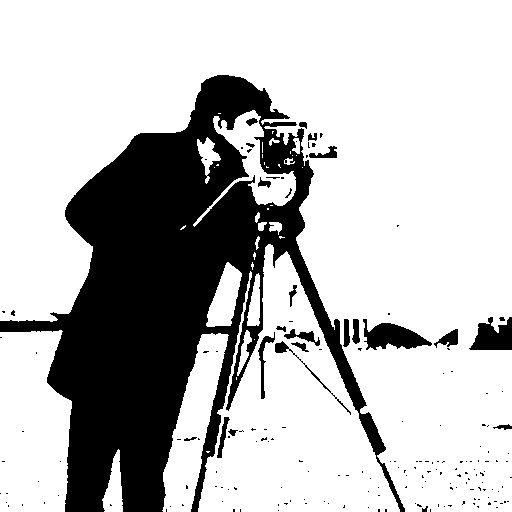
\includegraphics[interpolate=true,width=\textwidth]{images/essentials_binarization_window_size_otsu}
        \caption{Otsu's Methode\\(Global)}%
    \end{subfigure}
    \hfill
    \begin{subfigure}[t]{0.3\textwidth}
        \centering
        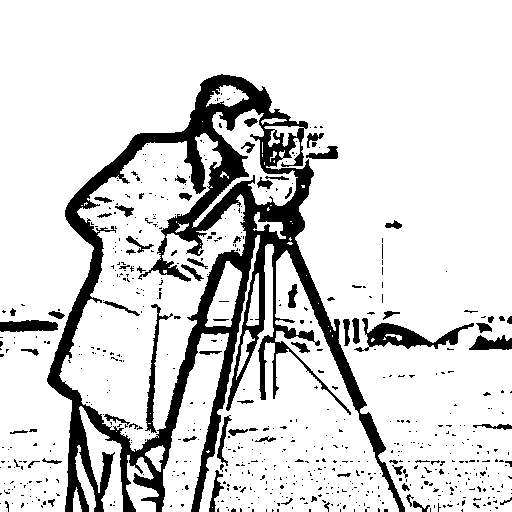
\includegraphics[interpolate=true,width=\textwidth]{images/essentials_binarization_window_size_sauvola}
        \caption{Sauvola's Methode\\(Lokal)}%
    \end{subfigure}
    \caption{Inkorrekte Binarisierung mit lokalen Schwellenwertfunktionen aufgrund zu kleiner Fenstergrößen}%
    \label{fig:essentials_binarization_window_size}
\end{figure}

\clearpage
\subsection{Sauvola's Methode}%
\label{subsec:essentials_binarization_sauvola}

Angenommen folgende Definitionen für Sauvola's Methode~\cite{DBLP:journals/pr/SauvolaP00} gelten:

\begin{tabu}{lX}
    \(w\)      & Fenstergröße des Algorithmus \\
    \(R\)      & Hälfte des Wertebereichs --- Beispielsweise \(128\) für 8-Bit Grafiken \\
    \(k\)      & Faktor des Einflusses der Standardabweichung auf den Schwellenwert \\
    \(m(x,y)\) & Durchschnittlicher Pixelwert im Fenster \((w,w)\) mit \((x,y)\) als Zentrum \\
    \(s(x,y)\) & Standardabweichung der Pixelwerte im Fenster \((w,w)\) mit \((x,y)\) als Zentrum \\
\end{tabu}

Dann wird der Schwellenwert wie folgt berechnet:
\begin{gather}
    T(x,y) = m(x,y) * \left(1 + k * \left(\frac{s(x,y)}{R} - 1\right)\right)
\end{gather}

Unter der Annahme, dass \(k\) ein kleiner, positiver Faktor ist, dann ist bereits ersichtlich wie
\begin{gather*}
    T(x,y) = m(x,y) * \ldots
\end{gather*}
mit dem durchschnittlichen Pixelwert \(m(x,y)\) die Gleichung dominiert und eine Art Basiswert für den Schwellenwert liefert.
\(m(x,y)\) wird im Fenster \((w,w)\) um das Zentrum \((x,y)\) berechnet, weshalb eine Änderung des durchschnittlichen Farbwertes über die Grafik hinweg auch eine Änderung des Schwellenwerts zur Folge hat.
Liegt demzufolge nur ein Teil eines Bildes im Schatten so passt sich Sauvola's Methode den neuen Umständen an.
Hierbei entsteht jedoch das Problem, dass in Bereichen geringer Farbwertvarianz innerhalb der Grafik die Schwelle fälschlicherweise bereits durch geringste Abweichungen unterschritten wird (\autoref{fig:essentials_binarize_without_stddev}).

Deshalb kommt nun die Standardabweichung \(s(x,y)\) zum Einsatz.
Da der Wertebereich der Standardabweichung dem Wertebereich der Grafik entspricht, folgt, dass
\begin{gather*}
    \frac{s(x,y)}{R} = 2
\end{gather*}
und somit der Gleichungsteil
\begin{gather*}
    k * \left(\frac{s(x,y)}{R} - 1\right)
\end{gather*}
einen Wertebereich von \([-k;+k]\) haben muss.

Dies wirkt in der Gleichung als Moderator, der den Schwellenwert, welcher auf dem durchschnittlichen Pixelwert \(m(x,y)\) basiert, um bis zu einem Faktor von \(k\) senken/erhöhen kann, falls die Standardabweichung der Pixel gering/hoch ist.
In Bereichen geringer Farbwertvarianz resultiert es darin, dass die Schwelle abgesenkt und somit nicht unterschritten wird (\autoref{fig:essentials_binarize_with_stddev}).

\begin{figure}[htbp]
    \begin{subfigure}[t]{0.3\textwidth}
        \centering
        
\includegraphics[interpolate=true,width=\textwidth]{images/smiley}
        \caption{Ursprüngliche Grafik}%
        \label{fig:essentials_binarize_input}
    \end{subfigure}
    \hfill
    \begin{subfigure}[t]{0.3\textwidth}
        \centering
        
\includegraphics[interpolate=true,width=\textwidth]{images/essentials_binarization_sauvola_without_stddev}
        \caption{Ohne Einfluss der Standardabweichung}%
        \label{fig:essentials_binarize_without_stddev}
    \end{subfigure}
    \hfill
    \begin{subfigure}[t]{0.3\textwidth}
        \centering
        
\includegraphics[interpolate=true,width=\textwidth]{images/essentials_binarization_sauvola}
        \caption{Mit Einfluss der Standardabweichung}%
        \label{fig:essentials_binarize_with_stddev}
    \end{subfigure}
    \caption{Binarisierung mittels Sauvola's Methode}%
    \label{fig:essentials_binarize}
\end{figure}

\clearpage
\section{Distanztransformation}%
\label{sec:essentials_distance_transform}

\begin{figure}[ht]
    \centering
    \begin{subfigure}[t]{0.45\textwidth}
        \centering
        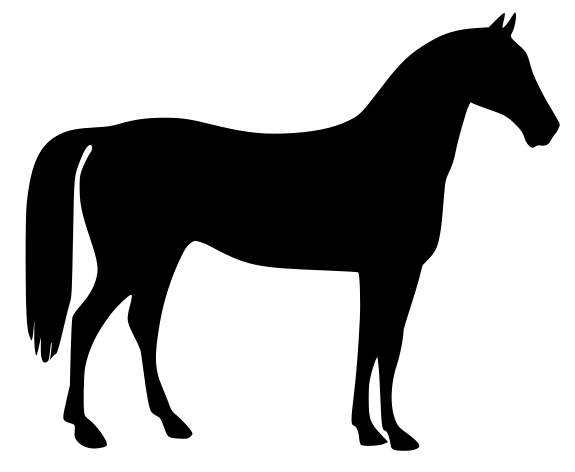
\includegraphics[interpolate=false,height=4cm]{images/holsteiner-stute}
    \end{subfigure}
    \hfill
    \begin{subfigure}[t]{0.45\textwidth}
        \centering
        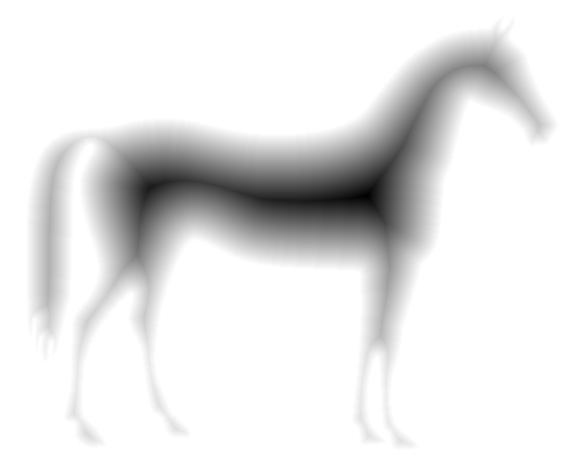
\includegraphics[interpolate=false,height=4cm]{images/essentials_distance_transform_horse}
    \end{subfigure}
    \caption{Eine euklidische Distanztransformation~\cite{DBLP:journals/pami/MaurerQR03,scikit-image}}%
    \label{fig:essentials_distance_transform_horse}
\end{figure}

\wrapfigurefix{0bp}
\begin{wrapfigure}{R}{4cm}
    \hyphenpenalty=0
    \centering
    \includesvg[inkscapelatex=false,inkscapearea=nocrop,width=4cm]{images/essentials_distance_transform}
    \caption{Distanztransformation eines Rechtecks}%
    \label{fig:essentials_distance_transform}
\end{wrapfigure}
Die Distanztransformation berechnet für jeden Vordergrundpixel die kürzeste Distanz zum Bildhintergrund~\cite{DBLP:journals/pr/RosenfeldP68}.
Solch eine Operation bildet die Grundlage für viele weiterführende Algorithmen --- unter anderem auch für die Medial-Achsen Transformation in \autoref{sec:essentials_skeletonization}.
Als Distanzfunktion wird in der Regel die euklidische Distanz benutzt.
Allerdings ist es auch möglich, andere Funktionen zu verwenden --- beispielsweise die Manhatten-Distanz.
\autoref{fig:essentials_distance_transform} zeigt die resultierenden Manhatten-Distanzen beispielhaft anhand eines zum Vordergrund zugehörigen Rechtecks.
\autoref{fig:essentials_distance_transform_horse} zeigt darüber hinaus analog eine euklidische Distanztransformation.
\wrapfigureunfix{}

Eine Brute-Force Berechnung der Distanztransformation ist hierbei ein sehr einfacher Ansatz, bei welchem für jeden Vordergrundpixel separat die geringste Distanz zu allen vorhandenen Hintergrundpixeln berechnet wird.
Solch eine Berechnung hat hierdurch jedoch eine Komplexität von \(\mathcal{O}(n^2)\) (\(n\): Pixelanzahl der Grafik).
Ein entsprechende, exemplarische Implementierung einer euklidischen Distanztransformation ist im Anhang in \autoref{lst:essentials_distance_transform_brute_force} sichtbar.

Im Implementationsteil dieser Arbeit wird später auf eine wesentlich komplexere und fortgeschrittenere Lösung in Form von Felzenszwalb's Methode~\cite{DBLP:journals/toc/FelzenszwalbH12} zurückgegriffen, welche von OpenCV~\cite{opencv_library} implementiert wurde.
Diese berechnet ebenfalls eine exakte euklidische Distanztransformation und liefert somit identische Ergebnisse zur Brute-Force Berechnung.
Anders als der Brute-Force Ansatz kann sie jedoch eine Komplexität von \(\mathcal{O}(n)\) und somit eine signifikant höhere Performanz vorweisen.

\clearpage
\section{Skelettierung}%
\label{sec:essentials_skeletonization}

\begin{figure}[ht]
    \begin{subfigure}[t]{0.48\textwidth}
        \centering
        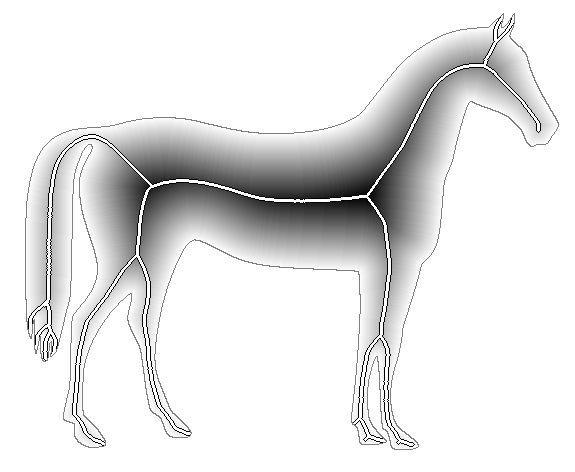
\includegraphics[interpolate=true,width=\textwidth]{images/essentials_skeletonize_medial_axis}
        \caption{Medial-Achsen Transformation, berechnet mit~\cite{scikit-image}}
    \end{subfigure}
    \hfill
    \begin{subfigure}[t]{0.48\textwidth}
        \centering
        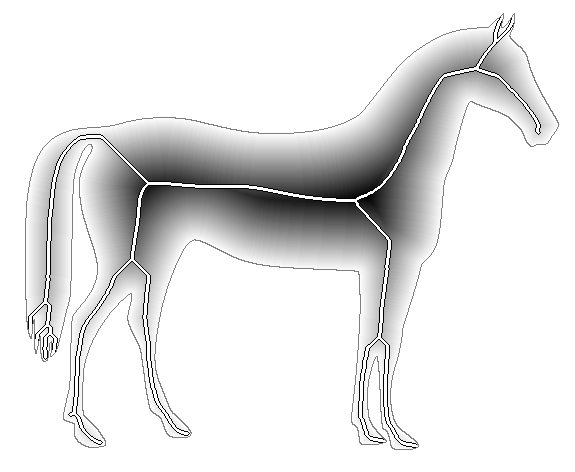
\includegraphics[interpolate=true,width=\textwidth]{images/essentials_skeletonize_thinning}
        \caption{Zhang-Suen Thinning~\cite{DBLP:journals/cacm/ZhangS84}}
    \end{subfigure}
    \caption[Gegenüberstellung zweier prinzipieller Ansätze der Skelettierung]{Gegenüberstellung zweier prinzipieller Ansätze der Skelettierung\\(die Distanztransformation der ursprünglichen Grafik ist im Hintergrund zu sehen)}%
    \label{fig:essentials_skeletonization_comparison}
\end{figure}

Bei der Skelettierung wird eine verdünnte Version einer binären Grafik erzeugt, welche nur noch aus annähernd ein Pixel breiten Linien besteht.
Generell ist es das Ziel, dass jeder Pixel des Skeletts sich möglichst gleich weit entfernt zu den jeweils nächstgelegenen, topologischen Rändern befindet.
Die zügige und gleichzeitig korrekte Ermittlung der Skelettierung in Binärgrafiken ist jedoch schwierig zu erreichen.
Existierende Algorithmen lassen sich deshalb mit zwei potentiellen Eigenschaften einordnen:
\begin{itemize}
    \item Geometrisch korrekt \\
    Das berechnete Skelett befindet sich exakt mittig zwischen den nächstgelegenen topologischen Rändern.
    Diese Eigenschaft bleibt auch dann beibehalten, wenn die Grafik rotiert, skaliert oder anderweitig transformiert wird.
    \item Topologisch korrekt \\
    Das Skelett behält die Topologie der ursprünglichen Grafik bei.
    Die Anzahl der verbundenen Komponenten der Grafik darf entsprechend nicht verändert werden.
\end{itemize}

Die Skelettierung mithilfe von Voronoi-Diagrammen~\cite{DBLP:conf/cvpr/OgniewiczI92} ist als Ausnahme in der Lage, beide Eigenschaften zu besitzen.
Deren Nutzung bleibt jedoch durch den hohen Rechenaufwand in der Regel verwehrt.
In der Praxis werden deshalb üblicherweise andere Herangehensweisen verwendet.

Eine geometrisch korrekte Skelettierung wird in der Regel auf Basis der Gebirgskämme einer Distanztransformation berechnet (siehe \autoref{sec:essentials_distance_transform}).
Solcherlei Herangehensweisen werden als \enquote{Medial-Achsen Transformation}~\cite{Blum:1967:ATF} bezeichnet.
Ein großes Problem ist jedoch die topologische Korrektheit derartiger Algorithmen, da es in der Praxis schwierig ist, alle relevanten Gebirgskämme der Distanztransformation zu extrahieren, ohne gleichzeitig die Skelettierung unnötig zu verkomplizieren.
Neuere Arbeiten fokussieren sich deshalb primär auf eine Verbesserung dieser Situation. (Beispielsweise~\cite{DBLP:journals/cg/MonteroL12}.)

Topologisch korrekte Skelettierungen können jedoch unter anderem mithilfe sogenanntem \enquote{Thinning}~\cite{DBLP:journals/pami/LamLS92} erhalten werden.
Derartige Algorithmen erodieren gezielt die ursprüngliche binäre Grafik sukzessiv, indem jeweils triviale Pixel entfernt werden.
\enquote{Triviale Pixel} sind hierbei jene, welche beim Entfernen nicht die Anzahl der verbundenen Komponenten ändern.
Da die Thinning-Algorithmen einzig die Konnektivität betrachten, kann jedoch zwangsläufig nicht mehr die geometrisch korrekte Platzierung der Skelettierung garantiert werden.

\autoref{fig:essentials_skeletonization_comparison} zeigt Beispielhaft die geometrische Korrektheit einer Medial-Achsen Transformation~\cite{scikit-image} gegenüber dem Zhang-Suen Thinning~\cite{DBLP:journals/cacm/ZhangS84}.

Die vorliegende Arbeit beschäftigt sich mit der Skelettierung von Handzeichnungen bei gleichzeitigem Erhalt der Linienbreite.
Als solches wird es im Entwurfsteil dieser Arbeit (siehe \autoref{cha:theory}) notwendig werden, die Distanztransformation der binarisierten Grafik zu berechnen.
Es ist deshalb naheliegend eine Medial-Achsen Transformation einzusetzen, welche direkt auf der bereits berechneten Distanztransformation aufbaut.
Diese würde darüber hinaus eine geometrisch korrekte Skelettierung und somit eine gute optische Repräsentation der ursprünglichen Grafik garantieren.
Moderne Algorithmen der Medial-Achsen Transformation (beispielsweise~\cite{DBLP:journals/cg/MonteroL12}) konnten in kleineren Testläufen auch stets topologisch korrekte Skelettierungen erzielen.
Jedoch stellte sich die Implementation solcher modernen Algorithmen als zu zeitaufwändig heraus, weshalb die Nutzung der Medial-Achsen Transformation verworfen wurde.
Im folgenden Abschnitt wird deshalb die gewählte, einfachere Alternative in Form des etablierten Zhang-Suen Thinning erläutert.

\subsection{Zhang-Suen Thinning}%
\label{subsec:essentials_skeletonization_zhang_suen}

\wrapfigurefix{0bp}
\begin{wrapfigure}{R}{5cm}
    \centering
    \includesvg[inkscapelatex=false,inkscapearea=nocrop]{images/essentials_zhang_suen_grid}
    \caption{Bezeichnung der Pixelnachbarschaft}%
    \label{fig:essentials_zhang_suen_grid}
\end{wrapfigure}
Einer der bekanntesten Thinning-Algorithmen ist Zhang-Suen's Methode~\cite{DBLP:journals/cacm/ZhangS84}.
Angenommen man betrachtet jedes Pixel \(P_1\) an der Stelle \((x,y)\) der Grafik in einem \((3,3)\) Fenster.
Die Werte der Pixel sind entweder \(0\) für den Bildhintergrund oder \(1\) für den zu erodierenden Bildvordergrund.
Die um \(P_1\) liegenden Pixel werden entsprechend \autoref{fig:essentials_zhang_suen_grid} benannt.
\wrapfigureunfix{}

Zhang-Suen's Methode wird nun sukzessiv triviale Pixel in der Grafik entfernen, beziehungsweise auf \(0\) setzen.
Der Vorgang wird solange wiederholt bis keine Pixel mehr erkannt und entfernt werden können.
Jede Iteration operiert hierbei in zwei sequentiellen Durchläufen.
Tatsächliche Mutationen werden jedoch auf die Grafik erst nach einem Durchlauf angewendet, wodurch es möglich wird den folgenden Algorithmus beliebig zu parallelisieren.

In beiden Durchläufen gilt generell, dass \(P_1\) ein triviales Pixel ist, falls:
\begin{align}
    \label{eq:essentials_zhang_suen_cond_p} & P_1 = 1 \\
    \label{eq:essentials_zhang_suen_cond_a} & A(P_1) = 1 \\
    \label{eq:essentials_zhang_suen_cond_b} & 2 \leq B(P_1) \leq 6
\end{align}
Wobei:
\begin{align}
    A(P_1) &= \text{Anzahl von }0 \to 1\text{ Übergängen in }(P_2, \ldots, P_9) \\
    B(P_1) &= P_2 + \cdots + P_9
\end{align}
Des Weiteren gilt im ersten Durchlauf:
\begin{align}
    \label{eq:essentials_zhang_suen_cond_1}
    \begin{split}
        P_2 * P_4 * P_6 &= 0 \\
        P_4 * P_6 * P_8 &= 0
    \end{split}
\end{align}
Sowie im zweiten Durchlauf:
\begin{align}
    \label{eq:essentials_zhang_suen_cond_2}
    \begin{split}
        P_2 * P_4 * P_8 &= 0 \\
        P_2 * P_6 * P_8 &= 0
    \end{split}
\end{align}

\autoref{eq:essentials_zhang_suen_cond_p} stellt sicher, dass nur Pixel betrachtet werden, welche noch zum Vordergrund gehören.
\autoref{eq:essentials_zhang_suen_cond_a} verhindert, dass \(P_1\) entfernt wird, falls hierdurch die Konnektivität des Skeletts reduziert werden würde (\autoref{fig:essentials_zhang_suen_cond_a}).
\autoref{eq:essentials_zhang_suen_cond_b} verhindert mithilfe von \(2 \leq B(P_1)\)  weiterhin, dass Linienenden unnötig gekürzt werden (\autoref{fig:essentials_zhang_suen_cond_b1}), sowie mit \(B(P_1) \leq 6\), dass fälschlicherweise Löcher in noch nicht vollständig skelettierten Bereichen erzeugt werden (\autoref{fig:essentials_zhang_suen_cond_b7}).

Diese Regelungen ergeben nun insgesamt \(40\) verschiedene Anordnungen in denen Pixel erodiert werden.
Für jede Anordnungen innerhalb der \(40\) lässt sich jeweils eine weitere erlaubte Anordnung finden welche horizontal und/oder vertikal gespiegelt ist (vergleiche \autoref{fig:essentials_zhang_suen_cond_both}, versus \autoref{fig:essentials_zhang_suen_cond_1}).
Jeder Durchlauf betrachtet jedoch jeweils nur \(34\) davon.
Dies ist eine besondere Notwendigkeit für Zhang-Suen Thinning, da aufgrund der \((3,3)\) Fenstergröße eine Situation entstehen kann, in welcher zwei oder mehr spiegelsymmetrische Anordnungen zu zwei oder mehr benachbarten Pixeln passen und somit eine ganze Guppe von Pixeln in einem einzelnen Durchlauf entfernt werden könnte.
Deshalb teilen \autoref{eq:essentials_zhang_suen_cond_1} und \autoref{eq:essentials_zhang_suen_cond_2} jede Iteration in zwei einzelne, eindeutige Durchläufe auf.
Dieser Umstand wird unter anderem in~\cite{DBLP:conf/icpr/ZhangW88a} diskutiert und der Algorithmus zu einem Durchlauf per Iteration verbessert.

\clearpage
\begin{figure}[!htb]
    \centering
    \begin{subfigure}[t]{0.3\textwidth}
        \centering
        \includesvg[inkscapelatex=false,inkscapearea=nocrop,height=1cm]{images/essentials_zhang_suen_both}
        \caption{In beiden Durchläufen zu entfernendes Pixel}%
        \label{fig:essentials_zhang_suen_cond_both}
    \end{subfigure}
    \hfill
    \begin{subfigure}[t]{0.3\textwidth}
        \centering
        \includesvg[inkscapelatex=false,inkscapearea=nocrop,height=1cm]{images/essentials_zhang_suen_first}
        \caption{Im ersten Durchlauf zu entfernendes Pixel}%
        \label{fig:essentials_zhang_suen_cond_1}
    \end{subfigure}
    \hfill
    \begin{subfigure}[t]{0.3\textwidth}
        \centering
        \includesvg[inkscapelatex=false,inkscapearea=nocrop,height=1cm]{images/essentials_zhang_suen_bad_a}
        \caption{Nicht zu entfernendes Pixel, da \(A(P_1) = 2\)}%
        \label{fig:essentials_zhang_suen_cond_a}
    \end{subfigure}

    \begin{subfigure}[t]{0.3\textwidth}
        \centering
        \includesvg[inkscapelatex=false,inkscapearea=nocrop,height=1cm]{images/essentials_zhang_suen_bad_b1}
        \caption{Nicht zu entfernendes Pixel, da \(B(P_1) = 1\)}%
        \label{fig:essentials_zhang_suen_cond_b1}
    \end{subfigure}
    \qquad
    \begin{subfigure}[t]{0.3\textwidth}
        \centering
        \includesvg[inkscapelatex=false,inkscapearea=nocrop,height=1cm]{images/essentials_zhang_suen_bad_b7}
        \caption{Nicht zu entfernendes Pixel, da \(B(P_1) = 7\)}%
        \label{fig:essentials_zhang_suen_cond_b7}
    \end{subfigure}
    \caption{Potentielle Anordnungen beim Zhang-Suen Thinning}
\end{figure}

\subsection{Imperfektionen des Zhang-Suen Thinning}%
\label{subsec:essentials_skeletonization_zhang_suen_imperfection}

\begin{wrapfigure}{R}{5cm}
    \centering
    \includesvg[inkscapelatex=false,inkscapearea=nocrop,height=1cm]{images/essentials_zhang_suen_imperfection}
    \caption{Imperfektion des Zhang-Suen Thinning}%
    \label{fig:essentials_zhang_suen_imperfection}
\end{wrapfigure}
Leider gehört Zhang-Suen Thinning zu jenen Skelettierungsalgorithmen, welche nicht exakt ein Pixel breite Linien erzeugen.
Anordnungen wie in \autoref{fig:essentials_zhang_suen_imperfection} sowie deren \(\lbrace{}90°,180°,270°\rbrace{}\) Rotationen, enthalten den überflüssigen Pixel \textunicode{▨}, welcher ohne Störung der Topologie entfernt werden könnte~\cite{DBLP:journals/pami/LamLS92}.

\clearpage
\section{Douglas-Peucker Kurvenglättung}%
\label{sec:essentials_douglas_peucker}

Der Douglas-Peucker Algorithmus~\cite{doi:10.3138/FM57-6770-U75U-7727} ist ein weit bekannter Ansatz zur Glättung beziehungsweise Approximation von Linienzügen.
Ein Linienzug zwischen zwei Punkten \(P_1\) bis \(P_n\) wird zu der direkten Geraden \(\overline{P_1 P_n}\) vereinfacht, wenn alle Punkte \((P_2, \ldots, P_{n-1})\) einen lotrechten Abstand zur direkten Geraden von höchstens \(d\) haben (siehe \autoref{fig:essentials_douglas_peucker_simple}).
Ist dies nicht der Fall, so wird der Punkt \(P_m\) mit dem größten lotrechten Abstand ermittelt und der Linienzug in die zwei Abschnitte \((P_1, \ldots, P_m)\) und \((P_m, \ldots, P_n)\) aufgeteilt.
Auf beide Abschnitte wird nun derselbe Algorithmus rekursiv angewendet (siehe \autoref{fig:essentials_douglas_peucker_split}).

\mbox{}

\begin{figure}[htbp]
    \centering
    \begin{subfigure}[t]{0.45\textwidth}
        \centering
        \includesvg[inkscapelatex=false,inkscapearea=nocrop,height=6cm]{images/essentials_douglas_peucker_simple}
        \caption{Der gesamte Linienzug befindet sich innerhalb der Grenze \(d\)}%
        \label{fig:essentials_douglas_peucker_simple}
    \end{subfigure}
    \hfill
    \begin{subfigure}[t]{0.45\textwidth}
        \centering
        \includesvg[inkscapelatex=false,inkscapearea=nocrop,height=6cm]{images/essentials_douglas_peucker_split}
        \caption{Ein Punkt \(P_m\) mit dem lotrechten Abstand \(m\) befindet sich außerhalb von \(d\)}%
        \label{fig:essentials_douglas_peucker_split}
    \end{subfigure}
    \caption{Visuelle Darstellung des Douglas-Peucker Algorithmus}
\end{figure}

\clearpage
\section{OpenCV}%
\label{sec:essentials_opencv}

OpenCV~\cite{opencv_library} steht für und ist eine \enquote{Open Source Computer Vision Library}.
Im Bereich der Bildverarbeitung gilt sie als eine allgemein bekannte und angesehene Bibliothek und bietet optimierte Implementationen einer Vielzahl an grundlegenden Imperativen sowie moderner Algorithmen.

Beispielsweise liest der folgende \texttt{C++} Code eine Bilddatei namens \texttt{input.jpg} ein, wendet den Gaußschen Weichzeichner mit einer Fenstergröße von \((3,3)\) an und speichert das Ergebnis als \texttt{output.jpg} ab:
\begin{minted}[gobble=4]{cpp}
    cv::Mat input = cv::imread("input.jpg");
    cv::Mat output;
    cv::blur(input, output, {3, 3});
    cv::imwrite("output.jpg", output);
\end{minted}

\texttt{cv::Mat} ist eine OpenCV Klasse, welche n-Dimensionale Matrizen verwaltet und steht in der Bibliothek an zentraler Stelle.
Liest man eine Bilddatei ein wird auch diese in einer solchen Matrix gespeichert (siehe Zeile 1).
So wie die meisten Funktionen in OpenCV ist dadurch auch die auf Zeile 3 verwendete \texttt{cv::blur} Funktion nur noch die abstrakte Transformation einer Matrix.

Zusätzlich bieten neuere Versionen von OpenCV die leicht abgewandelte Klasse \texttt{cv::UMat}.
Wird diese an Stelle von \texttt{cv::Mat} verwendet, können viele grundlegende Funktionen --- unter anderem auch \texttt{cv::blur} --- eine potentiell existierende GPU des Computers für eine starke Beschleunigung nutzen.

Da OpenCV nicht nur bereits zwei verschiedene Container-Klassen für Matrizen, sondern auch einige andere Formate unterstützen muss, sind die meisten Funktionen in OpenCV in etwa wie folgt definiert:
\begin{minted}[gobble=4]{cpp}
    void transformation(cv::InputArray source, cv::OutputArray destination);
\end{minted}

\texttt{cv::InputArray} speichert eine konstante Referenz zu einem der unterstützten Container-Klassen ab.
Es ist nachträglich möglich abzufragen, welche Art von Container das \texttt{cv::InputArray} speichert, weshalb die jeweilige Funktion sich zum Beispiel auf eine GPU-Beschleunigung spezialisieren kann, sofern der Aufrufer zur Laufzeit eine \texttt{cv::UMat} Instanz übergeben hat.
\texttt{cv::InputArray} stellt somit eine Art von manueller, dynamischer Polymorphie dar.

\texttt{cv::OutputArray} ist das entsprechende Gegenstück mit identischen Fähigkeiten.
Jedoch wird hierbei eine mutable Referenz gespeichert, in welcher das Ergebnis der Transformation gespeichert werden kann.
